\chapter{Exemples de QCM/Vrai ou Faux}

\begin{itemize}
\item Soit $A$ un problème appartenant à $DTIME(n^2)$ : % Q92
	\begin{itemize}
	\item $A \in P$
	\item $A \in DSPACE (n^2)$
	\item Il peut exister un programme Java de complexité $\bigO(n)$ qui décide $A$
	\item $A \in DTIME(n^3)$
	\end{itemize}
\item Si une fonction $f$ est calculable, alors toute fonction $g$ dont $f$ est une extension est calculable : \red{Faux} % Q41
\item Si le domaine d’une fonction est fini, alors cette fonction est calculable : \green{Vrai} % Q21
\item Si SAT $\leq_a A$ et $A \in P$, alors SAT $\in P$  : \red{Faux} % Q108
\item L’ensemble des sous-ensembles récursivement énumérables de $\mathbb{N}$ est énumérable : \green{Vrai} % Q18
\item Tout ensemble de paires d’entiers est récursif : \red{Faux} % Q17
\item L’ensemble des programmes Java calculant une fonction $f$ telle que $f(10)=10$ est un ensemble récursif : \red{Faux} % Q25
\item Un sous-ensemble infini d’un ensemble récursivement énumérable est récursivement énumérable : \red{Faux} % Q7
\item Soit $D$ un nouveau modèle de calculabilité. Si toute fonction calculable est calculable dans $D$ et si toute fonction calculable dans $D$ est effectivement calculable, alors $D$ est un modèle complet de la calculabilité : \red{Faux} % Q111
\item Un algorithme donné ne calcule qu’une et une seule fonction  : \green{Vrai} % Q12
\item Un sous-ensemble d’un ensemble récursivement énumérable est récursivement énumérable : \red{Faux} % Q19
\item Un problème qui peut être résolu par un algorithme (de complexité) exponentiel est pratiquement infaisable (intrinsèquement complexe) : \red{Faux} %Q84
\item Le complément d’un ensemble récursivement énumérable est récursivement énumérable : \red{Faux} %Q10
\item Soient les programmes $P_{32}(n)$ dont le code est « print(1) » et $P_{57}(n)$ dont le code est « print(0) » : %Q32
	\begin{itemize}
	\item Les fonctions $phi_{32}$ et $phi_{57}$ sont des fonctions constantes
	\end{itemize}
\item Les propriétés SA, CD et S sont suffisantes pour que D soit un modèle complet de la calculabilité : \green{Vrai} %Q113
\item Un ensemble est f-réductible (fonctionnellement réductible) à son complément : \red{Faux} %Q88
\item Si A peut être décidé par un algorithme polynomial et si B est f-réductible à A, alors B peut être décidé par un algorithme polynomial : \red{Faux} %Q89
\item Tout ensemble récursivement énumérable est a-réductible à HALT : \green{Vrai} %Q87
\item Un ensemble énumérable est récursif : \red{Faux} % Q2
\item Si A est un sous-ensemble (strict et non vide) récursif de programmes Java, alors toute fonction calculée par un programme de A est aussi calculée par un programme du complément de A : \red{Faux} %Q28
\item Soit A est un ensemble (infini) récursivement énumérable. Si B $\subseteq$ A, alors B est aussi récursivement énumérable : \red{Faux} %Q39
\item Il existe un ensemble infini de chaînes finies de caractères (A-Z) qui est non récursivement énumérable : \green{Vrai} % Q36
\item Une extension d’une fonction partielle calculable est toujours calculable : \red{Faux} % Q33
\item Le modèle de calcul BLOOP possède les propriétés SD et SA : \green{Vrai} % Q110
\item L’union d’une infinité énumérable d’ensembles récursivement énumérable est récursivement énumérable : \red{Faux} % Q9
\item Pour déterminer si un problème A est NP-complet, il suffit de déterminer que A est polynomialement réductible un problème NP-complet connu (e.g. SAT) : \red{Faux} % Q97
\item Il existe des ensembles récursifs qui ne sont pas récursivement énumérables : \red{Faux} % Q97
\item Un sous-ensemble infini d’un ensemble récursif est récursif : \red{Faux} % Q3
\end{itemize}

\chapter{Tests d'entrée aux TP 1 à 4}

\begin{itemize}
\item L'ensemble des nombres impairs positifs est énumérable. \green{Vrai}
\item L'ensemble des nombres premiers positifs est énumérable. \green{Vrai}
\item L'ensemble des nombres entiers est énumérable. \green{Vrai}
\item L'ensemble des nombres rationnels est énumérable. \green{Vrai}
\item L'ensemble des nombres irrationnels compris entre 0 et 1 est énumérable. \red{Faux}
\item L'ensemble des fonctions de $\mathbb{N}$ dans $\{0, 1\}$ est énumérable. \red{Faux}
\item L'ensemble des mots de longueur finie d'un alphabet énumérable est énumérable. \green{Vrai}
\item L'ensemble des mots d'une longueur infinie d'un alphabet énumérable est énumérable. \red{Faux}
\item Soit deux ensemble $A$ et $B$ avec la même cardinalité. Si $A$ n'est pas énumérable, alors $B$ ne l'est pas non plus. \green{Vrai}

\item L'ensemble des nombres premiers est récursif. \green{Vrai}
\item Un ensemble $X$ est récursif ssi $\bar{X}$ est récursif. \green{Vrai}
\item Soit deux ensembles récursifs $X$ et $Y$. $X \cup Y$, $X \cap Y$, et $\bar{X}$ sont récursifs. \green{Vrai}
\item Soit deux ensembles récursivement énumérables $X$ et $Y$. $X \cup Y$, $X \cap Y$, et $\bar{X}$ sont récursivement énumérables. \red{Faux}
\item La somme de deux fonctions calculables à une variable est toujours calculable. \green{Vrai}
\item Un ensemble $X$ est récursivement énumérable ssi il existe une fonction calculable partielle $f$ t.q. $X = dom(f)$. \green{Vrai}
\item Un ensemble $X$ est récursivement énumérable ssi il existe un programme Python qui énumère les éléments de $X$. \green{Vrai}
\item Un ensemble $X$ est récursivement énumérable ssi $X$ est l'ensemble vide où il existe une fonction totale calculable $f$ t.q. $X = im(f)$. \green{Vrai}

\item Soit $L$ un sous-ensemble récursif non trivial du langage Python qui ne permet de calculer que des fonctions totales. La fonction \textit{halt} de $L$ est calculable avec $L$. \green{Vrai}
\item Soit $L$ un sous-ensemble récursif non trivial du langage Python qui ne permet de calculer que des fonctions totales. La fonction \textit{halt} de $L$ est calculable avec Python. \green{Vrai}
\item Soit $L$ un sous-ensemble récursif non trivial du langage Python qui ne permet de calculer que des fonctions totales. La fonction interpréteur de $L$ est calculable avec $L$. \red{Faux}
\item Soit $L$ un sous-ensemble récursif non trivial du langage Python qui ne permet de calculer que des fonctions totales. La fonction interpréteur de $L$ est calculable avec Python. \green{Vrai}
\item Soit $L$ un sous-ensemble récursif non trivial du langage Python qui ne permet de calculer que des fonctions totales. Il existe une fonction totale calculable qui n'est pas calculable avec $L$. \green{Vrai}
\item Il existe un langage permettant de calculer à la fois sa fonction halt et sa fonction interpréteur. \green{Vrai}
\item Un ensemble non récursif ne peut pas être récursivement énumérable. \red{Faux}
\item Un ensemble non récursif ne peut pas être co-récursivement énumérable \red{Faux}
\item L'union de deux ensembles non récursifs est nécessairement non récursif. \red{Faux}
\item L'intersection de deux ensembles non récursif est nécessairement non récursif. \red{Faux}

\item L'ensemble des programmes qui calculent la fonction $f : \mathbb{N} \rightarrow \mathbb{N}$ t.q. $f(n) = 2n$ est récursif. \red{Faux}
\item L'ensemble des programmes qui renvoient 0 pour au moins une entrée est récursif. \red{Faux}
\item L'ensemble des programmes qui terminent après moins de 1000 instructions pour l'entrée 0 est récursif. \green{Vrai}
\item L'ensemble des programmes qui terminent pour au moins deux entrées différentes est récursif. \red{Faux}
\item L'ensemble des programmes qui calculent une fonction donnée $f : \mathbb{N} \rightarrow \mathbb{N}$ est récursif. \green{Vrai} si $f$ est non calculable, \red{Faux} sinon.
\item Il existe un programme Python qui décide si la fonction calculée par un programme donné a un domaine fini. \red{Faux}
\item L'ensemble $A = \{i | P_i(x)$ se termine pour un certain $x\}$ est récursif. \red{Faux}
\item L'ensemble $A = \{i \in \mathbb{N} | P_i(x)$ se termine pour un certain $x\}$ est récursivement énumérable. \green{Vrai}
\end{itemize}

\chapter{Vrai ou Faux avec justification}

\section*{Séance 1}

\begin{mcqs}
  \mcq{Certaines tâches ne peuvent pas être accomplies par un ordinateur}{1}
  {On ne peut pas implémenter les fonction non-calculables.}
  \mcq{Le langage Java est plus puissant que le langage C++}{0}
  {Hypothèse de l'équivalence des langages non-triviaux.}
  \mcq{Il est possible de détecter automatiquement certains virus sur un ordinateur}{1}
  {C'est ce que font les anti-virus, ils connaissent certains virus et ceux là ils les détectent.}
  \mcq{Il est possible de détecter automatiquement tout virus sur un ordinateur}{0}
  {Sinon drôle peut être implémenté et ça crée une contradiction.}
  \mcq{Un problème intrinsèquement complexe ne peut pas être résolu, même pour des petites données}
  {0}
  {Non, intrinsèquement complexe ne veut pas dire "non-calculable", il est exponentiel donc il est très lent mais résout le problème pour qui sait attendre.}
  \mcq{Grâce à l'évolution technologique, certains problèmes intrinsèquement complexes pourront être résolus dans quelques années}{0}
  {Peu importe les évolutions technologiques, un problème exponentiel (intrinsèquement complexe) ne peut et ne pourra être résolu que pour de petits exemples}
  \mcq{Les problèmes intrinsèquement complexes sont calculables}{1}
  {Par définition, ce sont des problèmes calculable dont tous les programmes qui les résolvent ont une complexité au moins exponentielle.}
  \mcq{Les problèmes non calculables sont intrinsèquement complexes}{0}
  {Par définition, un problème intrinsèquement complexe est calculable.}
\end{mcqs}

\section*{Séance 2}

\begin{mcqs}
  \mcq{L'ensemble des rationnels est énumérable}{1}
  {On peut les mettre dans un tableau 2D et les parcourir en zigzag.}
  \mcq{Un sous-ensemble infini d'un ensemble énumérable est énumérable}{1}
  {C'est un sous-ensemble donc il ne peut pas avoir plus d'éléments.}
  \mcq{Tout ensemble infini de chaînes finies de caractères est énumérable}{1}
  {S'il y a $k$ symbole, la bijection avec les entiers est immédiate si on considère la représentation de ces entiers en base $k$.}
  \mcq{Tout ensemble infini de chaînes infinies de caractères est énumérable}{0}
  {S'il y a $k$ symbole, la bijection avec les réels entre $[0,1]$ est immédiate si on considère la représentation des décimales de ces réels en base $k$.}
  \mcq{L'ensemble des fonctions de $\mathbb{N}$ vers $\{0,1\}$ est non énumérable}{1}
  {Considérons la chaîne infinie créée par $f(0)f(1)f(2)\cdots$. La bijection avec les réels entre $[0,1]$ est immédiate si on considère leur représentation des décimales de ces réels en binaire.}
  \mcq{L'ensemble des fonctions de $\{0,1\}$ vers $\mathbb{N}$ est énumérable}{1}
  {Représentons ces fonctions par le couple $(f(0),f(1))$.
  $f(0)$ et $f(1)$ sont entiers donc représentés de manière finie.
  Déjà on voit donc qu'on peut représenter les éléments de l'ensemble de manière finie, intuitivement c'est déjà énumérable.
  On voit tout de suite une surjection vers les rationnels $f(0)/f(1)$
  mais ça ne signifie pas qu'on a moins d'éléments que les rationnels car c'est pas injectif $2/2 = 1/1$.
  On peut remarquer cependant que c'est une union dénombrable d'ensemble dénombrables.
  C'est l'union des ensembles
  $\{\, (0,n) \mid n \in \mathbb{N} \,\},
   \{\, (1,n) \mid n \in \mathbb{N} \,\},
   \{\, (2,n) \mid n \in \mathbb{N} \,\},\ldots$.
  Une autre manière de le prouver, c'est en considérant le tableau où $f$ est à la ligne $f(0)$ et la colonne $f(1)$ et en parcourant le tableau en zigzag.}
  \mcq{Tout langage (alphabet fini) est énumérable}{0}
  {Comme les chaînes peuvent-être infinies. Par contre en informatique les chaînes sont finies donc VRAI dans ce cas.}
  \mcq{Toute fonction bijective est injective}{1}
  {Injectif: Ensemble d'arrivée n'est pas la cible de deux éléments de l'ensemble de départ; Bijectif: tous élément est cible de 1 et 1 seul.}
  \mcq{Une fonction dont la table est infinie ne peut être décrite de manière finie}{0}
  {$f \colon \mathbb{R}\rightarrow\mathbb{R} : f(x)=x^{2}$}
  \mcq{Toute fonction totale est surjective}{0}
  {$f \colon \R \to \R : f(x) = x^2$ n'est pas surjective car $\mathop{\mathrm{image}}(f) = \mathbb{R}^+$, les réels positifs mais $\mathop{\mathrm{dom}}(f) = \mathbb{R}$.}
  \mcq{Toute extension d'une fonction surjective est surjective}{1}
  {Tout ce qu'on fait c'est parfois changer l'output lorsqu'elle était $\bot$. On a donc au moins toutes les mêmes output qu'avant.}
  \mcq{Tout ensemble non-énumérable peut être mis en bijection avec l'ensemble des réels}{0}
  {Il existe des ensembles plus grands que l’ensemble des réels.}
  \mcq{L'ensemble des fonctions de $\mathbb{N}$ dans $\mathbb{N}$ est énumérable}{0}
  {On peut faire une diagonalisation.
  Chaque fonction est représentée dans une ligne par $f(0),f(1),f(2),\ldots$.
  On modifie simplement la diagonale en faisant $+1$.}
  \mcq{L'ensemble des programmes Java est énumérable}{1}
  {Le code Java est une chaîne finie sur un alphabet fini.}
  \mcq{L'énumérabilité des programmes Java et la non énumérabilité des fonctions de $\mathbb{N}$ vers $\mathbb{N}$ est une preuve de l'existence de fonctions non calculables}{1}
  {On peut définir une surjection des programmes vers les fonctions calculables qu'ils calculent.
  C'est une fonction car un programme calcule une seule fonction et c'est surjectif car toutes les fonctions calculables
  ont au moins un programme qui les calcule.
  On conclut qu'il y a un nombre énumérable de fonction calculable, c'est moins que le nombre de fonctions de $\mathbb{N}$ dans $\mathbb{N}$
  qui est non calculable, il y a donc des fonctions non calculables.}
  \mcq{L'ensemble des fonctions calculables est énumérable}{1}
  {Pour chaque fonction calculable, il existe un programme qui la calcule.
  Un programme ne calcule pas 2 fonctions différentes mais 2 programmes différents peuvent calculer une même fonction.
  Il n'y a donc pas plus de fonctions calculables que de programmes.
  Comme le nombre de programme est énumérable,
  il y a donc un nombre énumérable de fonction calculables.}
  \mcq{L'ensemble des fonctions non-calculables est énumérable}{0}
  {L'union de deux ensembles énumérables est énumérables.
  Seulement, l'union de l'ensemble des fonctions calculables et non-calculables
  est l'ensemble des fonctions de $\mathbb{N}$ dans $\mathbb{N}$ qui est non-énumérable.
  Comme l'ensemble des fonctions calculables est énumérable,
  l'ensemble des fonctions non-calculables ne peut pas être énumérable.}
\end{mcqs}

\section*{Séance 3}

\begin{mcqs}
  \mcq{Tout langage est récursif}{0}
  {Un langage est un ensemble de mots finis. Tous les ensembles d'entiers ne sont pas récursifs, car il y a autant de sous-ensembles de $\mathbb{N}$ qu'il y a d'éléments dans $\mathbb{R}$. Ils ne sont donc pas tous récursifs.}
  \mcq{Un ensemble énumérable est récursif}{0}
  {$\mathbb{K}$ est énumérable mais n'est pas récursif.}
  \mcq{Un sous-ensemble infini d'un ensemble récursif est récursif}{0}
  {$K$ est un sous ensemble de $\mathbb{N}$. $\mathbb{N}$ est récursif mais $K$ n'est pas récursif.}
  \mcq{Un ensemble fini est récursif}{1}
  {Si l'ensemble est fini, on peut créer un programme de taille finie qui gère l'entièreté des cas et donc dire s'il est ou non dans l'ensemble ($\Rightarrow$ récursif)}
  \mcq{Le complément d'un ensemble récursif est récursif}{1}
  {Il suffit d'appeler le programme de l'ensemble de départ et d'inverser la réponse.}
  \mcq{L'ensemble des rationnels est récursivement énumérable}{1}
  {On sait énumérer les rationnels avec un programme (tableau puis zigzag).}
  \mcq{Un sous-ensemble infini d'un ensemble récursivement énumérable est récursivement énumérable}{0}
  {Exemple : le complément de $K$ qui est bien un sous-ensemble infini de $\mathbb{N}$}
  \mcq{Un sous-ensemble fini d'un ensemble énumérable est récursivement énumérable}{1}
  {Un ensemble fini est récursif donc récursivement énumérable.}
  \mcq{L'union d'une infinité énumérable d'ensembles récursivement énumérable est récursivement énumérable}{1}
  {Supposons qu'on veut savoir si $x$ est dans l'union.
   Soient $A_1, A_2 \ldots$ ces ensembles et $f_1, f_2, \ldots$ leur fonctions d'énumération totales calculables.
   Faisons un tableau où sur la ligne $i$ on met $f_i(0), f_i(1), f_i(2), \ldots$.
   Parcourons le tableau en zigzag pour et à chaque fois qu'on arrive à la case $i,j$, on demande à $f_i$ le prochain élément
   de son énumération $f_i(j)$.
   Si c'est $f_i(j) = x$ alors $x$ est dans l'union et on renvoie 1.}
  \mcq{Le complément d'un ensemble récursivement énumérable est récursivement énumérable}{0}
  {Exemple: $K$}
  \mcq{Une fonction dont la table est infinie est non calculable}{0}
  {Exemple: $f(x) = x^2$}
  \mcq{Un algorithme donné ne calcule qu'une et une seule fonction}{1}
  {Un programme output toujours la même output pour le même input et détermine une seule et unique fonction.}
  \mcq{Il existe des ensembles non récursivement énumérables}{1}
  {Exemple: $\bar{K}$}
  \mcq{Une fonction calculable peut être calculée par une infinité de programmes\label{QCM:C3:3}}{1}
  {Il suffit de rajouter des lignes inutiles.}
  \mcq{L'ensemble HALT est récursivement énumérable}{1}
  {Avec l'input $n,x$ on exécute $n$ sur $x$ avec l’interpréteur universelle.
  S'il termine on renvoie $1$ sinon on ne termine pas mais ce n'est pas grave car on ne veut pas que le programme soit récursif.}
  \mcq{Il existe des ensembles récursifs qui ne sont pas récursivement énumérables}{0}
  {Être récursif est plus "dur" que d'être récursivement énumérable}
  \mcq{Tout ensemble de paires d'entiers est récursif}{0}
  {Par exemple l'ensemble $\{(n,x) \mid \mathit{halt}(n,x)=1\}$ n'est pas récursif}
  \mcq{L'ensemble des sous-ensembles récursivement énumérables de $\mathbb{N}$ est énumérable}{1}
  {Pour chaque sous-ensemble, il existe au moins un programme Java qui l'énumère et l'ensemble des programmes Java est énumérable.}
  \mcq{Un sous-ensemble d'un ensemble récursivement énumérable est récursivement énumérable}{0}
  {$\overline{K} \subseteq \mathbb{N}$. $\mathbb{N}$ est récursivement énumérable, $\overline{K}$ n'est pas récursivement énumérable.}
  \mcq{Il existe des ensembles récursifs qui ne sont pas énumérables}{0}
  {Tout ensemble récursif est énumérable. En informatique, on ne gère que les input qui peuvent être définie de manière finie
  donc on ne gère pas les ensemble non-énumérables.}
  \mcq{Si le domaine d'une fonction est fini, alors cette fonction est calculable\label{QCM:C3:1}}{1}
  {On peut hardcoder toute les image dans le programme et détermine laquelle on prend avec un \textit{case} sur l'input.}
  \mcq{Si le domaine d'une fonction est infini, alors cette fonction est non-calculable.\label{QCM:C3:2}}{0}
  {La fonction constante "$+1$" a un domaine infini mais elle est calculable}
  \mcq{Une fonction constante est toujours calculable}{1}
  {Par exemple "print 1, print 2, print 3, ..."}
  \mcq{Un programme Java calcule une infinité de fonctions}{0}
  {Il en calcule une seule.}
\end{mcqs}

\section*{Séance 4}

\begin{mcqs}
  \mcq{Le complément de l'ensemble $K$ est récursivement énumérable}{0}
  {Le complément de $K$ est co-récursivement énumérable. Si $K$ était récursivement énumérable et co-récursivement énumérable il serait énumérable.}
  \mcq{Il existe des ensembles non récursivement énumérables}{1}
  {Le complément de $K$}
  \mcq{Tout ensemble est récursivement énumérable ou co-récursivement énumérable}{0}
  {Chaque ensemble récursivement énumérable a un programme qui le décide donc il y a un nombre énumérable d'ensembles énumérables.
  Il y a au plus 2 fois plus d'ensembles récursivement énumérables ou co-récursivement énumérables que d'ensemble énumérables
  donc il y a un nombre énumérables d'ensemble récursivement énumérable ou co-récursivement énumérable.
  Hors il y a un un nombre non-énumérable de sous ensembles de $\mathbb{N}$.}
  \mcq{Soit la fonction $f(i) = 1$ si $\varphi_{i}(i) \neq \bot$, $f(i) = 0$ sinon. La fonction $f$ est calculable.}{0}
  {Sinon, on pourrait décider HALT.}
  \mcq{Soit la fonction $f(i) = 1$ si $\varphi_{i}(i) \neq \bot$, $f(i) = 0$ sinon. Le domaine de $f$ est récursif.}{1}
  {Nous travaillons avec un entier en input et en output, donc la fonction est $\mathbb{N} \rightarrow \mathbb{N}$.
  Le domaine est les input tels que l'output n'est pas $\bot$.
  Or $f$ ne renvoi jamais $\bot$ donc son domaine est $\mathbb{N}$ qui est récursif.}
  \mcq{Soit la fonction $f(i) = 1$ si $\varphi_{i}(i) \neq \bot$, $f(i) = 0$ sinon. L'image de $f$ est un ensemble récursif.}{1}
  {$\{0,1\}$ ne contient que deux entiers et est donc récursif}
  \mcq{$\varphi_{i}(i)$ dénote la fonction numéro $i$ (selon l'énumération choisie pour les fonctions)}{0}
  {$i$ est un numéro de programme}
  \mcq{Il existe un langage de programmation (non-trivial) dans lequel la fonction HALT est calculable}{1}
  {Mini-Java}
  \mcq{Il existe un langage de programmation (non-trivial) dans lequel on peut programmer la fonction HALT ainsi que l'interpréteur de ce langage.}{0}
  {Hoare-Allison}
  \mcq{Si un langage de programmation (non-trivial) permet de programmer son interpréteur, alors la fonction HALT est calculable dans ce langage}{0}
  {Mini-Java}
  \mcq{Il n'existe pas de langage de programmation (non-trivial) dans lequel toutes les fonctions calculées sont totales}{0}
  {La version mini-Java en est la preuve.}
  \mcq{Il n'existe pas de langage de programmation ne permettant de calculer que toutes les fonctions totales calculables}{1}
  {Théorème de Hoare-Allison}
  \mcq{Il existe une fonction totale calculable qui n'est l'extension d'aucune fonction partielle calculable}{0}
  {C'est très facile de créer une fonction partielle à partir d'une fonction totale.
  Il suffit de remplacer le retour d'une valeur par $\bot$. La fonction totale serait alors extension de la fonction partielle.}
  \mcq{Il existe une fonction partielle calculable telle qu'aucune fonction totale calculable n'est une extension de cette fonction partielle}{1}
  {Considérons le tableau avec à la ligne $i$, $\phi_i(0), \phi_i(1), \ldots$.
  Prenons la diagonale $\mathrm{diag}(k) = \phi_k(k)$.
  Considérons $\mathrm{diag\_mod}(k) = \phi_k(k)+1$.
  S'il existe un extension totale calculable $d_m$, soit $p$ le numéro d'un programme qui la calcule.
  Alors, on a un soucis en $d,d$.
  Si $\mathrm{diag}(d) = \bot$, $\phi_d(d) \neq \bot$ car $d$ est totale et donc $\mathrm{diag}(d) \neq \phi_d(d)$.
  Si $\mathrm{diag}(d) \neq \bot$, $\phi_d(d) = \mathrm{diag}(d) + 1 \neq \mathrm{diag}(d)$.}
\end{mcqs}

\section*{Séance 5}

\begin{mcqs}
  \mcq{L'ensemble des programmes Java calculant une fonction $f$ telle que $f(10)=10$ est un ensemble récursif.}{0}
  {Si ça concerne le comportement de la fonction, Rice nous dit que c'est impossible}
  \mcq{L'ensemble des programmes Java calculant une fonction $f$ telle que $f(10) = 10$ est un ensemble récursivement énumérable.}{1}
  {C'est vrai mais ce n'est pas un théorème, on lance le programme avec input 10.
  Si ça termine et que le résultat est 10, on renvoie 1. Ça n'a aucun lien avec Rice.}
  \mcq{Toute propriété relative aux programmes est non calculable.}{0}
  {Certaines propriétés concernant le programme (comme sa longueur ou sa syntaxe) sont calculables.}
  \mcq{Si $A$ est un sous-ensemble (strict et non-vide) récursif de programmes Java, alors toute fonction calculée par un programme de $A$ est aussi calculée par un programme du complément de $A$.}{0}
  {Tous les programmes de + de 10 lignes n'ont pas un équivalent de moins de 10 lignes. Il y a une différence entre $\forall$ et $\exists$, il en existe un mais ce n'est pas pour tous.}
  \mcq{La propriété S-m-n affirme que tout numéro de programme calculable peut être transformé en un numéro équivalent, mais avec moins de paramètres.}{0}
  {Il n'est pas équivalent, il ne marche que pour $m$ paramètres avec des valeurs précises.}
  \mcq{Les propriétés S-m-n et S sont équivalentes}{0}
  {Non, S-m-n est plus fort.}
  \mcq{Tous les langages de programmation satisfont la propriété S-m-n}{1}
  {Il suffit de spécialiser des paramètres,
  on sait faire ça dans tous les langages.}
\end{mcqs}

\section*{Séance 6}

\begin{mcqs}
  \mcq{Les propriétés S-m-n et S sont équivalentes}{0}
  {S-m-n $\Rightarrow$ S mais l'inverse n'est pas vrai.}
  \mcq{Tous les langages de programmation satisfont la propriété S-m-n}{1}
  {Voir QCM5.}
  \mcq{Le théorème du point fixe est une conséquence du théorème de Rice}{0}
  {L'inverse est vrai.}
  \mcq{Si deux programmes P1 et P2 calculent la même fonction, alors il existe un transformateur $f$ de programmes ($f$ fonction totale calculable), tel que $f$(P1)=P2.}{1}
  {Rien à voir avec le théorème du point fixe. La fonction constante P2 peut servir de $f$.}
  \mcq{Si $f$ est un transformateur de programmes ($f$ fonction totale calculable), alors il existe deux programmes P1 et P2 tels que $f$(P1)=P2 ainsi que P1 et P2 calculent la même fonction.}{1}
  {Point fixe}
  \mcq{Si $f$ est un transformateur de programmes ($f$ fonction totale calculable), alors il existe deux programmes P1 et P2 tels que $f$(P1)=P2 ainsi que P1 et P2 calculent la même fonction totale}{0}
  {Si $f$ remplace l'input par un programme qui fait juste une boucle, son output est toujours le même programme.
  Ce programme output tout le temps $\bot$ et ne peut donc pas être total.}
  \mcq{Le théorème du point fixe permet de démontrer que la fonction HALT est non calculable}{1}
  {Il peut tout démontrer : $K$ est non récursif, HALT est non récursif}
  \mcq{L'ensemble des nombres réels calculables est énumérable}{1}
  {Autant que de programmes}
\end{mcqs}

\section*{Séance 7}

\begin{mcqs}
  \mcq{Toutes les fonctions calculables par les programmes du langage BLOOP sont totales}{1}
  {Bloop se termine toujours}
  \mcq{Le langage BLOOP (Bounded Loop) ne permet de programmer que des fonctions totales. Il existe donc des fonctions totales calculables qui ne peuvent être programmées dans ce langage.}{1}
  {Hoare-Allison}
  \mcq{Tout ensemble ND-récursivement énumérable est récursif}{0}
  {Il est récursivement énumérable mais pas spécialement récursif.
  Par exemple, $K$ est récursivement énumérable et donc ND-récursivement énumérable mais n'est pas récursif.}
  \mcq{Il existe des ensembles récursifs ne pouvant être décidés par un automate fini}{1}
  {Dans un automate fini, tout s'arrête toujours. C'est donc toujours limité (Hoare-Allison)}
  \mcq{Tout automate à pile peut être représenté par un automate fini.}{0}
  {L'automate à pile apporte quelque chose de plus, il sait checker si un mot est de la forme $a^nb^n$ alors que l'automate fini ne sait pas le faire.}
  \mcq{Les grammaires sensibles au contexte permettent de définir plus de langages que les grammaires hors-contextes.}{1}
  {$a^nb^na^n$ ne peut être décrit par une grammaire hors contexte mais peut être décrit par une grammaire sensible au contexte.}
  \mcq{Les grammaires hors-contexte ne permettent de définir que des langages récursifs}{1}
  {Les grammaires hors contexte peuvent être parsée par des automates à piles qui se terminent toujours donc c'est récursif.}
  \mcq{Les grammaires sensibles au contexte ne permettent de définir que des langages récursifs.}{1}
  {Ça peut être parsé par des Machines de Turing à ruban fini.
  Comme le ruban est fini, il y a un nombre fini d'état possible.
  Il suffit d'exécuter cette machine de Turing et si elle retourne dans un même état, on sait qu'elle va boucler à l'infini
  et donc on la kill et on renvoi 0.}
  \mcq{Tout langage reconnu par un automate fini peut être reconnu par un automate à pile}{1}
  {Un automate fini est un automate à pile qui n'utilise pas sa pile.}
  \mcq{Tout langage récursif peut être décrit par une grammaire hors contexte}{0}
  {$a^nb^na^n$ est récursif mais ne peut pas être décrit par une grammaire hors contexte.}
  \mcq{Tout automate fini non déterministe peut être transformé en un automate fini déterministe équivalent}{1}
  {Pour le faire, on regroupe les différents états où on pourrait être en un seul état.
  Un état contient donc plusieurs état.}
\end{mcqs}

\section*{Séance 8}

\begin{mcqs}
  \mcq{Une Machine de Turing est un modèle abstrait ne pouvant pas être exécuté.}{0}
  {Il est aisé de faire un interpréteur de machine de Turing en Java.}
  \mcq{Une Machine de Turing dont le ruban serait fini à gauche ne serait pas un modèle complet de la calculabilité}{0}
  {Si les cases sont numérotées $[..., -2, -1, 0, 1, 2 ...]$ on peut les réarranger comme suit: $[0, 1, -1, 2, -2, ...]$}
  \mcq{Une Machine de Turing dont les seuls mouvements de la tête de lecture serait à droite ne serait pas un modèle complet de la calculabilité.}{1}
  {On serait pas lire ce qu'on écrit donc ça ne sert à rien d'écrire.
  Du coup ça revient à l'automate fini.}
  \mcq{Une Machine de Turing ne calcule que des fonctions totales.}{0}
  {Il est possible de boucler}
  \mcq{Soit $A$ un ensemble récursivement énumérable mais non récursif. Une Machine de Turing avec $A$ comme oracle est plus puissante qu'une machine de Turing sans oracle.}{1}
  {Car $A$ devient récursif.}
  \mcq{Une machine de Turing universelle nécessite l'utilisation d'au moins trois rubans}{0}
  {L'ajout de rubans est seulement une question de facilité ; il est toujours possible de revenir à un seul ruban.}
  \mcq{Toute fonction T-calculable est effectivement calculable.}{1}
  {À ce jour, on ne connaît rien d'implémentable qui calcule plus que ce qui est effectivement calculable.}
  \mcq{Une machine de Turing non déterministe permet de calculer plus de fonctions}{0}
  {On peut simuler toutes les exécutions du programme non déterministe à l'aide d'une machine de Turing déterministe.
  On sera beaucoup plus lent bien entendu mais ça on s'en fout lorsqu'on parle de calculabilité.
  L'invention de machine non-déterministe de changerait donc rien à la calculabilité.}
  \mcq{Soit une machin de Turing T qui reçoit en entrée une représentation d'une machin de Turing et qui fournit (toujours) comme résultat une représentation d'une machine de Turing. Il existe deux machines de Turing T1 et T2 tel que
    \begin{enumerate}
      \item l'exécution de T sur la représentation de T1 donne pour résultat T2 ;
      \item T1 et T2 calculent la même fonction
    \end{enumerate}
  }{1}
  {Point fixe}
\end{mcqs}

\section*{Séance 9}

\begin{mcqs}
  \mcq{Les fonctions primitives récursives sont toujours des fonctions totales.}{1}
  {Elles sont équivalents aux fonctions calculées par le langage BLOOP/Mini-Java}
  \mcq{Il existe des fonctions totales calculables qui ne sont pas primitives récursives}{1}
  {Hoare-Allison, l'interpréteur}
  \mcq{Toute fonction calculable peut être calculée par une fonction récursive}{1}
  {Modèle complet grâce à la minimisation}
  \mcq{Toute fonction calculable peut être calculée par une expression lambda}{1}
  {Modèle complet}
  \mcq{Toute expression lambda possède au moins une forme réduite}{0}
  {Il est possible que il y ait une boucle infinie dans la réduction et que on arrive jamais à une forme réduite (= que on ne sait plus réduire).
  C'est le cas par exemple de $(\lambda x\,(xx)\ \lambda x\,(xx)$)}
  \mcq{Le lambda calcul est un modèle complet de la calculabilité}{1}
  {Modèle complet}
  \mcq{Le lambda calcul est un modèle théorique sans utilité pratique}{0}
  {Très subjectif cependant.}
\end{mcqs}

\section*{Séance 10}

\begin{mcqs}
  \mcq{Si une fonction est calculable par une Machine de Turing, alors cette fonction est calculable par un programme Java}{1}
  {Ils sont tous les deux des modèles complets}
  \mcq{Le modèle de calcul BLOOP possède les propriétés SD et SA.}{1}
  {BLOOP est tout à fait Sound, il est juste pas Complete.}
  \mcq{Soit $D$ un nouveau modèle de calculabilité. Si toute fonction calculable est calculable dans D et si toute fonction calculable dans D est effectivement calculable, alors D est un modèle complet de la calculabilité.}{0}
  {Il manque l'aspect concret de réalisation.
  On a juste CD et SD mais pas U, S, CA ni SA.}
  \mcq{Un formalisme D de calculabilité possède la propriété U (description universelle) lorsque l'interpréteur de D est calculable.}{0}
  {Pour satisfaire U, il faut que l'interpréteur soit \textbf{D}-calculable.}
  \mcq{Les propriétés SA, CD et S sont suffisantes pour que D soit un modèle complet de la calculabilité.}{1}
  {$SA \Rightarrow SD$, $SA \land CD \Rightarrow U$ et $CD \land S \Rightarrow CA$.}
  \mcq{La calculabilité est une discipline née après l'apparition des ordinateurs.}{0}
  {La calculabilité et ses principaux résultats sont antérieurs à l'informatique.}
\end{mcqs}

\section*{Séance 11}

\begin{mcqs}
  \mcq{Si la complexité temporelle d'un algorithme est $\bigO(n^{2})$, alors elle est aussi $\bigO(n^{3})$}{1}
  {$(n^2) \in \bigO(n^3)$ et $\bigO$ est transitif.}
  \mcq{Si la complexité spatiale d'un algorithme est $\bigO(n^{3})$, alors elle ne peut pas être $\bigO(n^{2})$}{0}
  {$\bigO(n^{3})$ est une borne supérieure mais ça peut être moins!}
  \mcq{Un algorithme de complexité $\bigO(n^{2})$ est toujours plus rapide qu'un algorithme de complexité $\bigO(n^{3})$}{0}
  {Déjà c'est juste des bornes, peut être que le deuxième est $\bigO(n)$.
  Aussi c'est une complexité de pire cas, sur certains input, le deuxième est peut être plus rapide mais si dans le pire cas il est plus lent.
  Il y a également la constante, peut être que devant le $n^3$ il y a une petite constant, sur des petites inputs le deuxième est alors quand même plus rapide dans le pire cas.}
  \mcq{Un problème qui peut être résolu par un algorithme (de complexité) polynomial est pratiquement faisable.}{1}
  {Pratiquement faisable = Polynomial}
  \mcq{Un problème qui peut être résolu par un algorithme (de complexité) exponentiel est pratiquement infaisable}{0}
  {Il peut très bien être réalisable à la fois par un algorithme exponentiel ET un algorithme polynomial.}
  \mcq{Si un problème est intrinsèquement complexe en MT alors il est aussi intrinsèquement complexe pour le langage Java.}{1}
  {Le choix du modèle de calculabilité impacte la complexité temporelle. Néanmoins, la différence de complexité est tout au plus polynomiale entre tous les modèles de calcul déterministes. Or, la composition de fonctions polynomiales reste polynomiale!}
  \mcq{Un ensemble est a-réductible (algorithmiquement réductible) à son complément.}{1}
  {Dire que A est a-réductible à B signifie que l'algorithme pouvant décider B nous permet de décider A. Ici, décider le complément permet bien évidemment de décider l'ensemble initial, il suffit d'inverser la réponse.}
  \mcq{Tout ensemble récursivement énumérable est a-réductible à HALT.}{1}
  {Halt est le ``plus difficile''. Pour tout ensemble récursivement énumérable $A$, il existe un programme $P$ qui renvoie 1 si $x$ est dans $A$. Pour décider si $x \in A$, on demande à HALT si $P$ termine avec l'input $x$. Si oui, alors on renvoi $P(x)$, sinon on renvoi que $x$ n'appartient pas à $A$.}
  \mcq{Un ensemble est $f$-réductible (fonctionnellement réductible) à son complément.}{0}
  {La plupart du temps, il n'est pas possible de trouver une fonction qui transforme une instance d'un ensemble en une instance de son complément. Par exemple ensemble PAIR est $f$-réductible à IMPAIR. Il suffit de rajouter 1. Mais ce n'est pas nécessairement toujours possible...
  De plus si $A \leq_f B$ et $B$ est récursivement énumérable alors $A$ est récursivement énumérable.
  Si un ensemble est $f$-réductible à son complément ça voudrait donc dire que si $A$ est récursivement énumérable son complément l'est aussi.
  Seulement si un ensemble et son complément sont récursivement énumérables alors il est récursif.
  Ça voudrait donc dire que tout ensemble récursivement énumérable est récursif et donc HALT est récursif, absurde tout ça non ?}
  \mcq{Si $A$ peut être décidé par un algorithme polynomial et si $B$ est $f$-réductible à $A$, alors $B$ peut être décidé par un algorithme polynomial.}{0}
  {Parce que ce que la $f$-réductibilité veut dire : on peut décider $B$ en donnant $f(x)$ (on veut décider si $x$ est dans $B$) à $A$.
  Mais calculer $f(x)$ peut être avoir une complexité exponentielle.}
\end{mcqs}

\section*{Séance 12}

\begin{mcqs}
  \mcq{Si $A$ est dans $DTIME(n^{2})$, alors $A$ est dans $DSPACE(n^{2})$}{1}
  {Il faut au moins $n^2$ instructions pour accéder à $n^2$ cases.}
  \mcq{Si $A$ est dans $NTIME(n^{2})$, alors $A$ est dans $DTIME(n^{2})$}{0}
  {Il faut au moins que $A \in DTIME(c^{n^2})$. $n^2$ est la profondeur maximale de l'arbre. Si on simule le ND, alors on doit faire un bfs dans un arbre de profondeur $n^2$.}
  \mcq{Si $A \in NTIME(f)$ alors $A\in DTIME(f)$}{0}
  {Il faut au moins que $A \in DTIME(c^f)$. f est la profondeur maximale de l'arbre. Si on simule le ND, alors on doit faire un bfs dans un arbre de profondeur f.}
  \mcq{Si $A \in NTIME(n^{2})$ alors $A \in NP$}{1}
  {$n^2$ est polynomial donc c'est non-déterministe polynomial.}
  \mcq{S'il existe un algorithme Java de complexité temporelle $\bigO(n^{2})$ décidant l'ensemble $A$, alors il existe une machine de Turing de complexité temporelle $\bigO(n^{2})$ décidant l'ensemble $A$.}{0}
  {Pas de transfert de complexité entre formalismes. On peut seulement dire que la MT va résoudre le problème en un temps polynomial. On ne peut pas assurer $\bigO(n^{2})$}
  \mcq{Le choix d'un modèle de calculabilité n'influence pas la classe $DTIME(n^{2})$}{0}
  {$n^2$ en Java ne veut pas dire $n^2$ en MT, juste polynomial.}
  \mcq{Si $A \leq_{p} B$ alors $A \leq_{a} B$.}{1}
  {Car la réduction polynomiale, en plus d’avoir une réduction algorithmique, on a aussi une information sur la complexité
  et même si on ne sait pas si $P$ est strictement inclus dans $NP$ on connaît des algorithm exponentiels non-polynomiales.}
  \mcq{La classe P est strictement inclue dans la classe EXPTIME.}{1}
  {Aucun problème polynomial n'est plus dur qu'un problème exponentiel.}
  \mcq{Tout problème calculable est au moins dans exptime.}{0}
  {Il existe pire comme la fonction d'Ackerman}
  \mcq{Un problème NP-complet peut toujours être décidé par un programme non déterministe de complexité polynomiale.}{1}
  {C'est la définition de NP}
  \mcq{Le problème du voyageur de commerce est NP-complet.}{1}
  {Le problème du cycle Hamiltonien est réductible au TSP et Richard M. Karp a montré en 1972 que le problème du cycle Hamiltonien est NP-complet.}
\end{mcqs}

\section*{Séance 13}

\begin{mcqs}
  \mcq{Un problème NP-complet est intrinsèquement complexe.}{2}
  {On en sait rien (intrinsèquement complexe = qui n'a pas d'algorithme polynomial) Vrai si $P \neq NP$ et Faux si $P=NP$.}
  \mcq{Le choix d’un modèle de calculabilité n’influence pas les classes P et NP.}{1}
  {Ça n'influence pas les classes (indépendante des langages).}
  \mcq{Le problème de la programmation linéaire est NP-complet.}{0}
  {La programmation linéaire est dans P (ensemble d'inéquations linéaire avec une fonction objectif linéaire qu'on veut optimiser).
  C'est résolu en temps polynomial par l'interior point method inventée par Yurii Nesterov (UCL) et Arkadi Nemirovski (Georgia Tech).}
  \mcq{Un problème de décision dans P, alors le problème consistant à calculer une solution est également dans P.}{1}
  {Pourquoi la complexité ferait des choses qui ne servent à rien ? Si on se focalise sur un problème de décision, c'est pcq c'est plus facile à traiter d'un point de vue théorique mais dans la pratique ça ne change rien! Donner la réponse si on sait qu'elle existe ça ne change rien.}
  \mcq{Un problème intrinsèquement complexe est dans EXPTIME.}{0}
  {Il y a des complexités pire qu'exponentielle.}
  \mcq{Un problème NP-complet peut être résolu par un algorithme non déterministe de complexité temporelle polynomiale.}{1}
  {La question qui met dehors à un examen oral.}
  \mcq{Un problème NP-complet peut être résolu par un algorithme non déterministe de complexité spaciale polynomiale.}{1}
  {La complexité spatiale est toujours bornée par la complexité temporelle.}
  \mcq{Si SAT${}\in{}$P, alors P$\subseteq$NP.}{1}
  {P est dans NP de toute façon mais si SAT $\in$ P alors P${}={}$NP.}
  \mcq{Si $SAT \in P$, alors P${}={}$NP.}{1}
  {SAT est NP-complet, tout problème NP est polynomialement réductible à lui.}
  \mcq{Si SAT $\leq_{a}$ A et $A \in P$, alors SAT $\in$ P.}{0}
  {On a besoin de la réduction polynomiale et pas la réduction algorithmique}
\end{mcqs}

\chapter{Anciens examens}

\section{Juin 2019}

\subsection*{Machine de Turing}

\begin{figure}[H]
    \centering
    \legend{Soit la machine de Turing suivante avec $\Sigma = \{0,1\}$}
    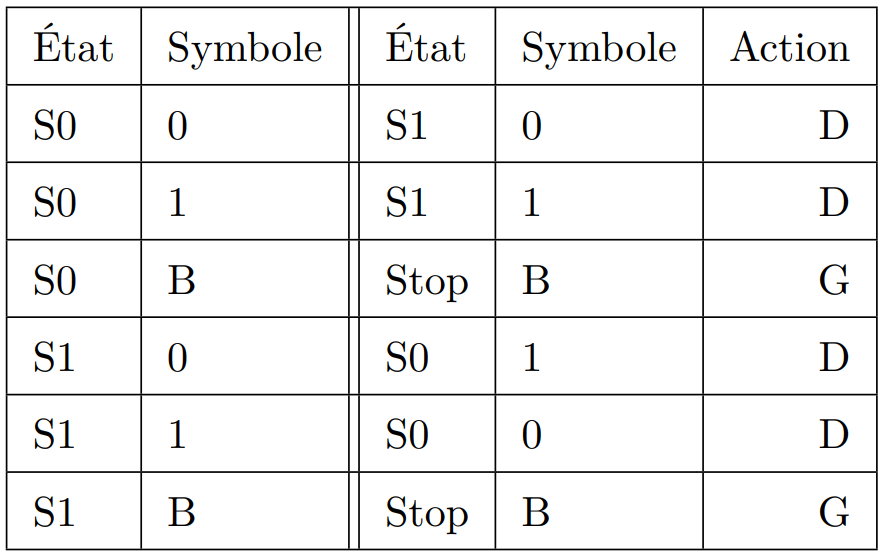
\includegraphics[width=0.3\textwidth,keepaspectratio]{mtJuin2019}
\end{figure}

\textbf{Machine déterministe ?} Vrai/Faux $\rightarrow$ \textit{Vrai, une seule exécution possible pour une entrée donnée}

\textbf{Machine a 2 états ?} Vrai/Faux $\rightarrow$ \textit{Faux, 3 états : $S_0, S_1$, et Stop}

\textbf{Sortie pour entrée 110011 ?} $\rightarrow$ \textit{$100110$}

\subsection*{Questions vrai/faux avec justification}

\begin{mcqs}
  \mcq{L’ensemble des fonctions de $\mathbb{N}$ vers $\{0,1\}$ est non énumérable.}{1}
  {Vrai (même principe que pour \ref{sec:ensembleF})}
  \mcq{Il n’existe pas de langage tel que \emph{halt} est calculable dans ce langage.}{0}
  {Faux, \emph{BLOOP} en est un exemple : tous les programmes de \emph{BLOOP} se terminent donc \emph{halt} retourne simplement 1}
  \mcq{Un sous ensemble infini d’un ensemble récursivement énumérable est récursivement énumérable.}{0}
  {Le complément de $K$ est bien un sous-ensemble infini de $\mathbb{N}$ mais n'est pas récursivement énumérable.}
  \mcq{Le théorème du Point Fixe est une conséquence du théorème de Rice.}{0}
  {L'inverse est vrai, le théorème de Rice est une conséquence du théorème du Point fixe.}
  \mcq{Une grammaire hors contexte ne permet que de construire des langages récursifs.}{1}
  {Les grammaires hors contexte peuvent être parsée par des automates à piles qui se terminent toujours (donc récursif).}
  \mcq{Un formalisme \(D\) qui a un interpréteur calculable possède la propriété U.}{0}
  {Faux, il doit aussi avoir la propriété CA, ou encore les propriétés CD et S.}
  \mcq{Si $A \in NP$ et $A \le_{p} SAT$ alors $A$ est NP-Complet.}{1}
  {Faux, il faut que SAT $\leq_p$ A, pas l'inverse.}
\end{mcqs}

\subsection*{Énoncer précisément le théorème de Rixe, donner sa signification et ses conséquences}

Voir \ref{dem:Rice}.

\subsection*{Définir la réduction polynomiale et prouver que si $SAT \in P$, alors $P = NP$}

Voir \ref{dem:PNP}.

\newpage
\section{Juin 2021}

\subsection*{Déterminer quelles sont les affirmations vraies}

\begin{enumerate}
\item Si le domaine d'une fonction est fini, alors cette fonction est calculable\\
	\green{Vrai} : voir \ref{QCM:C3:1}
\item Si le domaine d'une fonction est infini, alors cette fonction est non calculable\\
	\red{Faux} : voir \ref{QCM:C3:2}
\item Une fonction calculable est toujours calculée par une infinité de programme Java\\
	\green{Vrai} : voir \ref{QCM:C3:3}
\end{enumerate}

\subsection*{Déterminer pour chacun des ensembles suivants s'il est récursif, récursivement énumérable (mais non récursif) ou non récursivement énumérable}

\begin{enumerate}
\item $A = \{\ n\ |$ pour la donnée $5$, $P_n$ donne un entier pair comme résultat $\}$\\
	\blue{Récursivement énumérable mais non récursif}
\item $B = \{\ n\ |$ pour la donnée $5$, $P_n$ ne donne pas un entier pair comme résultat $\}$\\
	\blue{Non récursivement énumérable}
\end{enumerate}

\subsection*{Déterminer quelles sont les affirmations vraies}

Soit $A$ l'automate fini suivant, avec $\Sigma = \{0, 1\}, S_0 =$ état initial

\begin{figure}[H]
    \centering
    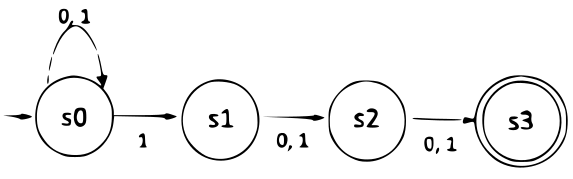
\includegraphics[width=0.35\textwidth,keepaspectratio]{juin2021Q3}
\end{figure}

\begin{enumerate}
\item $A$ est un automate fini déterministe\\
	\red{Faux}
\item Tous les strings de longueur strictement inférieur à $3$ sont non acceptés\\
	\green{Vrai}
\item Le string $101010$ est accepté\\
	\red{Faux}
\end{enumerate}

\subsection*{Pour chacune des affirmations ci-après, déterminer si celle-ci est vraie ou fausse. Ensuite vous devez justifier votre réponse.}

\begin{mcqs}
  \mcq{L'ensemble des fonctions de $\{0, 1\}$ vers $\mathbb{N}$ est non énumérable.}{0}
  {À chaque $\varphi_n$ est associé une paire d'entiers finis ($\varphi_n(0), \varphi_n(1)$). Un tableau de dimensions $\infty$x$2$ est énumérable.}
  \mcq{un sous-ensemble d'un ensemble récursif différent de $\mathbb{N}$ est récursif.}{0}
  {Soit $M$ l'ensemble récursif des entiers impairs. $M \neq \mathbb{N}$ et $A = \{\ n\ |\ \varphi_n$ est injectif et $n \in M\}$. $A \subseteq M$, mais par le théorème de Rice, il ne peut pas être récursif.}
  \mcq{Soit le langage de programmation BLOOP (où tous les programmes se terminent). Il est impossible de programmer en Java la fonction halt de BLOOP \textbf{et} l'interpréteur de BLOOP}{0}
  {halt de BLOOP peut être écrit en Java (avec "System.out.println("1");"). Java est un modèle complète de calculabilité (contrairement à BLOOP) et donc un interpréteur universel peut être écrit en Java.}
  \mcq{Une Machine de Turing dont les seuls mouvements de la tête de lecture sont à droite n'est pas un modèle complet de la calculabilité.}{1}
  {Cela revient à faire un automate à états finis qui ne peut pas lire ce qu'il a écrit.}
  \mcq{Si $f$ est une fonction totale calculable, alors il existe $x$ tel que pour tout $k : \varphi_k(x) = \varphi_{f(k)}(x)$.}{0}
  {Le théorème du point fixe dit qu'il existe un $k$ tel que pour tout $k : \varphi_k(x) = \varphi_{f(k)}(x)$ (en supposant $f$ totale calculable).}
  \mcq{Soit $D$ un nouveau modèle de calculabilité. Si toute fonction calculable est calculable dans $D$, si l’interpréteur de $D$ est calculable et si $D$ possède la propriété $S$, alors $D$ est un modèle complet de calculabilité.}{0}
  {Il manque les propriétés SA, SD et U dans le modèle $D$ pour qu'il soit un modèle complet de calculabilité.}
  \mcq{P $\subseteq$ PSPACE}{1}
  {La complexité spatiale ne peut excéder la complexité temporelle mais puisqu'on suppose qu'un algorithme efficace ne prend pas plus d'une case mémoire par instruction, P $=$ PSPACE}
\end{mcqs}

\subsection*{Compléter le théorème de Rice}

Voir \ref{dem:Rice}.

\subsection*{Déterminer quelles clauses peuvent être obtenues en appliquant une fois la règle de résolution}

Soient les clauses $\neg A \vee B \vee \neg D \vee F$ et $\neg B \vee C \vee \neg F$.

\begin{enumerate}
\item $\neg A \vee C \vee \neg D \vee F \vee \neg F$
\item $B \vee \neg B \vee F \vee \neg F$
\item $\neg A \vee B \vee \neg B \vee C \vee \neg D$
\item $\neg A \vee C \vee \neg D$
\item True
\end{enumerate}

\textit{Réponse} : 1 et 3.

\subsection*{Quelles sont les affirmations équivalentes à $p \models q$ ($q$ est une conséquence logique de $p$ ?}

\begin{enumerate}
\item $p \Rightarrow q$ est une tautologie
\item $p \Rightarrow q$ est satisfaisable
\item $p \Rightarrow q$ est non satisfaisable
\item Tous les modèles de $p$ qui sont aussi des modèles de $q$
\item Il existe un modèle de $p$ qui est aussi un modèle de $q$
\item $(p \wedge \neg q)$ est non satisfaisable
\end{enumerate}

\textit{Réponse} : 1, 4 et 6.

\subsection*{Déterminer quelles sont les affirmations qui sont vraies}

Soit $A \in$ DTIME($n^2$) :
\begin{enumerate}
\item $A \in$ DTIME($n^3$)
\item $A \in$ NTIME($n^2$)
\item Il n'existe aucun programme Java de complexité \bigO($n$) qui décide A
\item Il peut exister un programme Java de complexité \bigO($n$) qui décide A
\item $A \in P$
\end{enumerate}

\textit{Réponse} : 1, 2, 4 et 5.

\subsection*{Démonter que si SAT $\in P$, alors $P=NP$}

Voir \ref{dem:PNP}.
